\chapter{Espacios topológicos}%
\label{cha:espacios_topologicos}

\section{Conjuntos abiertos}%
\label{sec:conjuntos_abiertos}
\begin{defi}
Una \underline{topología} en un conjunto $X$ es una colección $\mathcal{T} \subset \mathcal{P}\left( x \right)$ de subconjuntos tal que:
\begin{enumerate}
    \item $\emptyset, X \in \mathcal{T}$ 
    \item Las uniones arbitrarias de elementos de $\mathcal{T}$ están en $\mathcal{T}$.
    \item Las intersecciones \underline{finitas} de elementos de $\mathcal{T}$ están en $\mathcal{T}$.
\end{enumerate}
Se dice que $\left( X, \mathcal{T} \right)$ es un \underline{espacio topológico}, los elementos de $\mathcal{T}$ se llaman \underline{abiertos} y los elementos de $X$ se llaman \underline{puntos}. 
\end{defi}

\begin{ej}
\begin{enumerate}
    \item \label{ejemplos_topologia:first} $\mathcal{T} = \{\emptyset, X\}$ es la llamada topología \underline{trivial}. $\mathcal{T} = P\left( X \right)$ es la topología \underline{discreta}: como los puntos $\{x\} \in \mathcal{T}$, entonces cualquier $A = \bigcup_{x \in A} \{x\}$ es abierto.
    \item $\mathbb{R}^n$ con la topología usual definida mediante las bolas euclídeas.
    \item Cualquier distancia $d$ define una topología mediante sus bolas abiertas, igual que se define la usual. \underline{Notación}: 
    \[
    B\left( a, \varepsilon \right) = \{d\left( a, x \right) < \varepsilon\},\ B\left[ a, \varepsilon \right] = \{d\left( a, x \right) \le \varepsilon \},\ S\left[ a, \varepsilon \right] = \{d\left( a, x \right) = \varepsilon\} 
    \]
    \item En un conjunto se pueden definir muchas topologías distintas (por ejemplo (\ref{ejemplos_topologia:first})) pero se puede asumir que solo ``parezcan'' distintas. Ya se sabe que la topología usual de $\mathbb{R}^n$ se puede definir mediante muchas distancias distintas.

    %TODO: Dibujo
    \begin{center}
        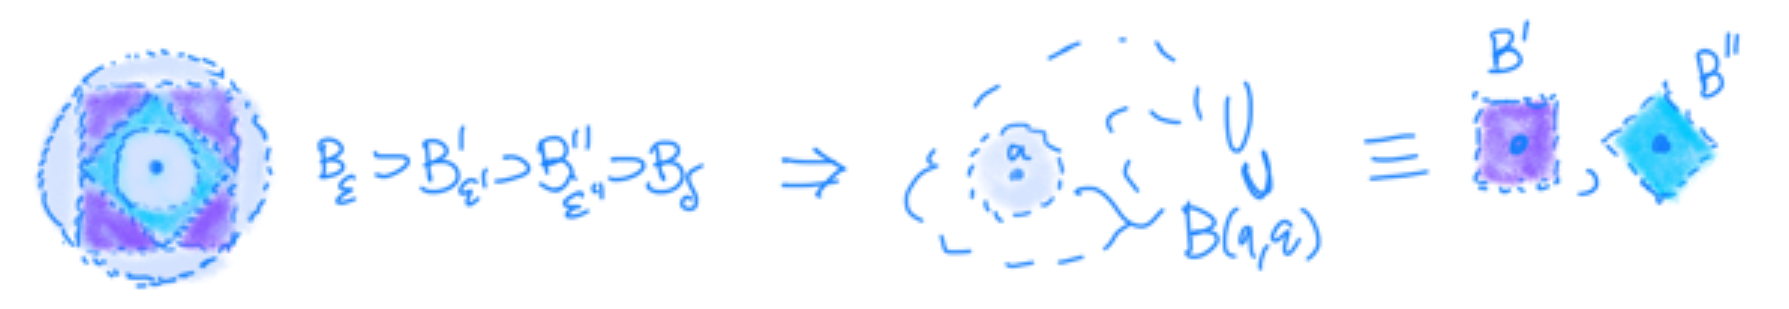
\includegraphics[scale=0.2]{images/topologia_metricas}  

        \textit{El dibujo representa distintas distancias\footnote{Procedentes de \textit{normas}.} en $\mathbb{R}^n$, pero todas definen la misma topología.} 
    \end{center}
    \item Una topología para ilustrar muchas propiedades (y contraejemplos). 

    Fijamos $a \in X$:
    \[
    \mathcal{T}_a = \{U \subset X: a \in U\} \cup \{\emptyset\} 
    \]
    La topología ``del punto''. El punto $\{a\}$ y todos los pares de puntos $\{a, x\}$ son abiertos. Se parece a la discreta pero difiere en que en esta última todos los puntos son abiertos.
\end{enumerate}
\end{ej}

Ya que en mismo conjunto podemos equiparlo con diversas topologías, es natural compararlas.
\begin{defi}
Dos topologías: $\mathcal{T}_1 \subset \mathcal{T}_2$ en $X$ se llaman \underline{comparables}: $\mathcal{T}_2$ es más ``fina'' que $\mathcal{T}_1$.
\end{defi}
Siempre se da:
\[
\mathcal{T}_{\text{trivial}} \subset \mathcal{T} \subset \mathcal{T}_{\text{discreta}} 
\]
Sea $\left( X, \mathcal{T} \right)$ un espacio topológico; a menudo se omite $\mathcal{T}$ ó el calificativo ``topológico''. 

\begin{defi}
\begin{enumerate}
    \item Un \underline{entorno abierto} de un punto $x \in X$ es un abierto $U$ que lo contiene. Se suele escribir $U^x$.
    \item Un \underline{entorno} de un punto $x \in X$ es un conjunto $V$ que contiene un abierto $U$ que contiene al punto. Se suele escribir $V^x$.\footnote{La intersección finita de entornos es entorno. (Si son abiertos es trivial)}
\end{enumerate}
\end{defi}
%TODO: Fix imagen
\begin{center}
    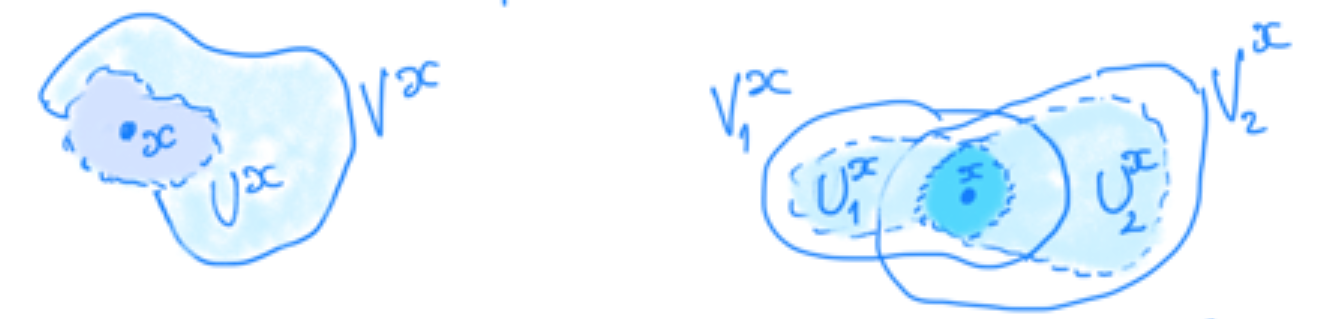
\includegraphics[scale=0.2]{images/def_entornos} 
\end{center}
\begin{obs}    
\begin{enumerate}
    \item Con $U^x \subset V^x$:
    \begin{align*}
        V_1^x \cap V_2^x &= V^x\\
        U_1^x \cap U_2^x &= U_{\text{ab}}^x \ni x
    \end{align*}

    %TODO: Corregir esta observación
    \item $U \in \mathcal{T}$ es entorno de todos \underline{sus} puntos.
    \begin{demo}
    \[
    x \in U \text{ abierto} \subset U
    \]
    \end{demo}
\end{enumerate}
\end{obs}

\begin{defi}
Sea $A \subset X$. Un \underline{punto interior de $A$} es un punto del que $A$ es entorno (luego $A$ lo contiene). El \underline{interior de $A$} es el conjunto de sus puntos interiores:
\[
\inter_X \left( A \right) = \mathring{A} = \{x \in A: \exists U^x \stackrel{\text{ab.}}{\subset}  A\} 
\]
\end{defi}
%TODO: Fix imagen
\begin{center}
    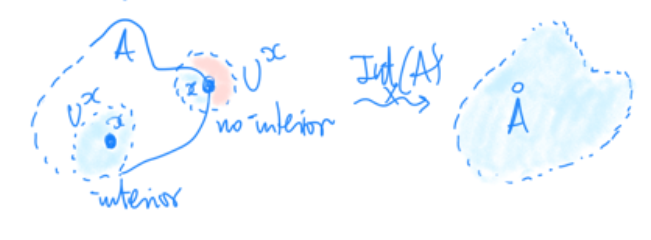
\includegraphics[scale=0.4]{images/def_interior} 
\end{center}

\begin{prop}
$\mathring{A}$ es el mayor abierto contenido en $A$: 
\[
\mathring{A} = \bigcup_{U \stackrel{\text{ab.}}{\subset} A} U
\]
En particular, $A$ abierto $\Leftrightarrow A = \mathring{A} \Leftrightarrow A$ es un entorno de todos los puntos.    
\end{prop}
\begin{demo}
\begin{enumerate}
    \item $\mathring{A}$ es abierto: 
    \begin{gather*}
        \begin{rcases}
        \forall x \in \mathring{A} &\Rightarrow \exists U^x \stackrel{\text{ab.}}{\subset}  A\\
        \forall y \in U^x &\Rightarrow A \supset U^x \text{ es un abierto que contiene a } y \Rightarrow y \in \mathring{A}.\\
        \end{rcases} \Rightarrow U^x \subset \mathring{A}\\
        \Rightarrow \mathring{A} = \bigcup_{x \in \mathring{A}} U^x \text{ es abierto como unión de abiertos}
    .\end{gather*}
    \item $\mathring{A}$ es el mayor abierto contenido en $A$.
    \[
    U \stackrel{\text{ab.}}{\subset} A \Rightarrow \forall x \in U \subset A \Rightarrow x \in \mathring{A} \Rightarrow U \subset \mathring{A} 
    \]
\end{enumerate}
\end{demo}

\begin{ej}
\begin{enumerate}
    \item $\left( X, \mathcal{T}_{\text{trivial}} \right): A \neq X \Rightarrow A \not \supset X \Rightarrow \emptyset$ es el único abierto $\subset A \Rightarrow \mathring{A} = \emptyset$.

    \item En $\mathbb{R}^n$ con $\mathcal{T}_{\text{trivial}}$ ya lo sabemos bien:
    \[
    \inter\left( B\left[ a, \varepsilon \right] \right)  = B\left( a, \varepsilon \right);\ \mathring{\mathbb{Q}}^n = \emptyset;\ \mathring{\mathbb{Z}}^n = \emptyset
    \]
    \item Si $a \in X,\ \mathcal{T}_a : \mathring{\{a\}} = \{a\};\ x \neq a,\ \mathring{\{x\}} = \emptyset$.
\end{enumerate}
\end{ej}

\begin{prop}
\begin{enumerate}
    \item $A \subset B \Rightarrow \mathring{A} \subset \mathring{B}$.
    \item $\mathring{A} \cap \mathring{B} = \inter \left( A \cap B \right)$.
\end{enumerate}
\end{prop}
\begin{demo}
\begin{enumerate}
    \item $A \subset B \Rightarrow \mathring{A} \subset A \subset B$ y $\mathring{A}$ es abierto $\Rightarrow \mathring{A} \subset \mathring{B}$. 
    \item 
    \begin{gather*}
    \begin{rcases}
    \begin{cases}
        \mathring{A} \cap \mathring{B} \text{ abierto (intersección finita de abiertos)}\\
        \mathring{A} \cap \mathring{B} \subset A \cap B 
    \end{cases} &\Rightarrow \mathring{A} \cap \mathring{B} \subset \inter \left( A \cap B \right)\\
    A \cap B \subset A, B \xRightarrow{1.} \inter \left( A \cap B \right) \subset \mathring{A}, \mathring{B} &\Rightarrow \inter\left( A \cap B \right) \subset \mathring{A} \cap \mathring{B}
    \end{rcases} \Rightarrow\\
    \boxed{\mathring{A} \cap \mathring{B} = \inter\left( A \cap B \right)} 
    .\end{gather*}
\end{enumerate}
\end{demo}

\section{Conjuntos cerrados}%
\label{sec:conjuntos_cerrados}
Sea $\left( X, \mathcal{T} \right)$ un espacio topológico.
\begin{defi}
Un conjunto \underline{cerrado} es un subconjunto $F \subset X$ tal que $U = X \setminus F$ es abierto.
\end{defi}
\begin{obs}
    Cerrado \underline{no} significa ``no abierto'', hay conjuntos que no son ni abiertos ni cerrados.
    %TODO: Fix imagen
    \begin{center}
        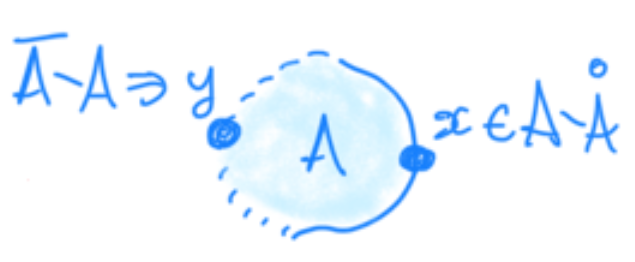
\includegraphics[scale=0.3]{images/def_cerrados} 
    \end{center}
\end{obs}
\begin{prop}
Se cumple que, $\mathcal{F} = \{\text{cerrados}\}$:
\begin{enumerate}
    \item $X, \emptyset$ son cerrados.
    \item La intersección arbitraria de cerrados es cerrada.
    \item La unión finita de cerrados es cerrado.
\end{enumerate}
\begin{demo}
    Porque $\bigcap_{i \in  I} \left( X \setminus U_i \right) = X \setminus \bigcup_{i \in I}^n U_i$ y $\bigcup_{i = 1}^n X \setminus U_i = X \setminus \bigcap_{i = 1}^n U_i$. Que son abiertos por ser unión arbitraria e intersección finita.
\end{demo}
\end{prop}

\begin{ej}
\begin{enumerate}
    \item En la topología trivial solo son cerrados $\emptyset$ y $X$. En la discreta, todos los subconjuntos son cerrados.
    \item En $\mathbb{R}^n$ con la topología usual ya sabemos todos los ejemplos: $B\left[ a, \varepsilon \right] : \lVert x - a \rVert \le \varepsilon$.
    \item Si $\mathcal{T}_1 \subset \mathcal{T}_2$, todo cerrado de $\mathcal{T}_1$ es cerrado de $\mathcal{T}_2$. (Cuidado con el orden) 
\end{enumerate}
\end{ej}

Para saber cuándo se aleja un conjunto de ser cerrado tenemos:
\begin{defi}
Sea $A \subset X$. Un punto \underline{adherente} a $A$ es un punto cuyos entornos intersecan todos a $A$. La \underline{adherencia} de $A$ es el conjunto de sus puntos adherentes. 
\[
\adh_X\left( A \right) = \overline{A} = \{x \in X: \forall V^x \cap A \neq \emptyset\} \supset A
\]
\end{defi}

\begin{obs}
Las primeras fórmulas importantes son:
\begin{gather*}
    \boxed{X \setminus \overline{A} = \inter\left( X \setminus A \right)} \\
    \boxed{X \setminus \mathring{B} = \overline{X \setminus B}} 
.\end{gather*}
\begin{demo}
\begin{itemize}
    \item $x \in X \setminus \overline{A} \Leftrightarrow x \not\in \overline{A} \Leftrightarrow \exists U^x \cap A = \emptyset \Leftrightarrow \exists U^x \subset X \setminus A \Leftrightarrow x \in \inter\left( X \setminus A \right)$
    \item $x \not\in \mathring{B} \Leftrightarrow \nexists U^x \subset B \Leftrightarrow \forall U^x \cap \left( X \setminus B \right) \neq \emptyset \Leftrightarrow x \in \overline{X \setminus B}$.
\end{itemize}
\end{demo}
\end{obs}

\begin{prop}
$\overline{A}$ es el menor cerrado que contiene a $A$: 
\[
    \boxed{\overline{A} = \bigcap_{F \stackrel{\text{cerr.}}{\supset} A} F } 
\]

En particular, $A$ cerrado $\Leftrightarrow \overline{A} = A \Leftrightarrow A$ contiene todos sus puntos de adherencia.
\end{prop}
\begin{demo}
$\overline{A} = X \setminus \inter\left( X \setminus A \right) = X \setminus \underbrace{\bigcup_{U \subset X \setminus A} U = X \setminus \bigcup_{F \supset A}}_{F = X \setminus U} \left( X \setminus F \right) = \bigcap_{F \supset A} F$.
\end{demo}

\begin{obs}
Lo anterior nos implica:
\begin{itemize}
    \item $B \supset A \Rightarrow \overline{B} \supset B \supset A \Rightarrow \overline{B} \supset \overline{A}$.
    \item $\overline{A \cup B} = \overline{A} \cup \overline{B}$:
    \[
    \begin{cases}
        \overline{A\cup B} \supset A \cup B \supset \begin{cases}
            A\\B
        \end{cases} \Rightarrow \overline{A\cup B} \supset \begin{cases}
            \overline{A} \\ \overline{B} 
        \end{cases} \Rightarrow \overline{A\cup B} \supset \overline{A} \cup \overline{B}\\

        A \cup B \subset \overline{A} \cup \overline{B} \Rightarrow \overline{A\cup B} \subset \overline{A} \cup \overline{B} 
    \end{cases} 
    \]
    La última implicación por que es cerrado al ser la unión de dos cerrados.
\end{itemize}
\end{obs}

\begin{ej}
\begin{enumerate}
    \item En $\mathbb{R}^n, \mathcal{T}_{\text{usual}}: B\left[ a, \varepsilon \right] = \overline{B \left( a, \varepsilon \right)};\ \overline{\mathbb{Q}^n} = \mathbb{R}^n$.
    \item $a \in X, \mathcal{T}_a$
    \[
        \begin{cases}
        \overline{\{a\}} = X \left[ \forall x, \forall U^x \supset \{a, x\} \ni a \Rightarrow x \in \overline{\{a\}} \right]\\
        x \neq a, \overline{\{x\}} = \{x\} \left[ y\neq x \Rightarrow U^y = \{a, y\} \cap \{x\} = \emptyset \right] 
        \end{cases} 
    \]
\end{enumerate}
\end{ej}

\begin{defi}[Otros puntos especiales]    
\begin{enumerate}
    \item $x$ es un \underline{punto aislado} de $A$ si $\exists V^x \cap A = \{x\}$.
    \item $x$ es un \underline{punto de acumulación} de $A$ si $\forall V^x \cap A \setminus \{x\} \neq \emptyset$. Y, evidentemente,
    \[
    \overline{A} = \{\underbrace{\text{puntos aislados}}_{\subset A}\} \sqcup \{\underbrace{\text{puntos de acumulación}}_{\supset \overline{A} \setminus A}\} 
    \]
    \item $x$ es un \underline{punto frontera} de $A$ si es adherente a $A$ y a $X \setminus A$, o bien, si no es interior de $X \setminus A$ ni de $A$. La \underline{frontera} de $A$ es: 
    \[
    \fr\left( A \right) = \{x \in X: x \text{ es punto frontera de } A\} = \overline{A} \cap \overline{X \setminus A} = \overline{A} \setminus \mathring{A}     
    \]
\end{enumerate}
\end{defi}

\begin{ej}
\begin{enumerate}
    \item En $\mathbb{R}, \mathcal{T}_u$ todos los puntos de $\mathbb{Z}$ son aislados, $\fr\left( \mathbb{Z} \right) = \mathbb{Z}$.
    \item En $\mathbb{R}^n, \mathcal{T}_u: \fr\left( B\left( a, \varepsilon \right) \right) = \fr\left( B\left[ a, \varepsilon \right] \right) = S\left[ a, \varepsilon \right] : \lVert x - a \rVert = \varepsilon$.
    \item En $\mathcal{T}_{\text{discreta}}$ todos los puntos son aislados, todas las fronteras son vacías.
    \item $a \in X, \mathcal{T}_a: $
    \[
    \begin{cases}
        \fr\left( \{a\} \right) = \overline{\{a\}} \setminus \mathring{\{a\}} = X \setminus \{a\}\\
        x \neq a, \fr\left( \{x\} \right) = \overline{\{x\}} \setminus \mathring{\{x\}} = \{x\} 
    \end{cases} 
    \]
\end{enumerate}
\end{ej}

Ahora, un concepto importante:
\begin{defi}
$A \subset X$ es \underline{denso} si $\overline{A} = X$, o bien, todo punto es adherente a $A$, o bien, todo abierto $\left( \neq \emptyset \right)$ corta a $A$.
\end{defi}

\begin{ej}
\begin{enumerate}
    \item $\mathbb{Q} \subset \mathbb{R}, \mathcal{T}_{\text{usual}}; \mathbb{Q} \times \overbrace{\ldots}^{n} \times \mathbb{Q} \subset \mathbb{R}^n, \mathcal{T}_{\text{usual}}$ son densos.
    \item $\{a\}$ es denso en $\left( X, \mathcal{T}_a \right)$.
\end{enumerate}
\end{ej}

\section{Bases}%
\label{sec:bases}
Sea $X, \mathcal{T}$ un espacio topológico.
\begin{defi}
Una \underline{base de entornos} de $a \in X$ es una colección $\mathcal{V}^a$ de entornos de $a$, tal que todo entorno de $a$ contiene uno de $\mathcal{V}^a$.
\end{defi}

\begin{obs}
No se supone ninguna propiedad especial, ni que sean abiertos. Veremos que la existencia de base de entornos con propiedades adicionales es una de las cosas que determinan el comportamiento de la topología.

Pero, $\forall \mathcal{V}^a$ se puede \underline{refinar} a una base $\mathcal{B}^a$ de entornos de abiertos. 
\begin{demo}    
\[
\forall V^a \in \mathcal{V}^a,\ \exists U^a \subset V^a \Rightarrow \mathcal{B}^a = \{U^a: V^a \in \mathcal{V}^a\} \text{ es base de entornos}. \left[ \forall E^a \supset V^a \supset U^a \right] 
\]
\end{demo}
\end{obs}

\begin{pg}
    Bastan las bases de entornos para comprobar propiedades de todos los entornos.
\end{pg}

\begin{il}    
Por ejemplo,
\begin{align*}
    a \in \overline{A} &\xLeftrightarrow{\text{def}} \forall W^a \text{ entorno }: W^a \cap A \neq \emptyset\\
   &\Longleftrightarrow \forall V^a \in \mathcal{V}^a: V^a\cap A \neq \emptyset 
.\end{align*}
\end{il}

\begin{ej}
\begin{enumerate}
    \item $\mathbb{R}^n, \mathcal{T}_{\text{usual}}: $
    \[
    \begin{cases}
    \mathcal{B}^a = \{B\left( a, \varepsilon \right): \varepsilon > 0\} \text{ base de entornos abiertos.}  \\
    \mathcal{V}^a = \{B\left[ a, \varepsilon \right]: \varepsilon > 0\} \text{ base de entornos cerrados.} 
    \end{cases} 
    \]
    \item $a \in X, \mathcal{T}_a : \mathcal{B}^a = \{\{a\}\},\ \mathcal{B}^x = \{\{a, x\}\},\ x \neq a$.
\end{enumerate}
\end{ej}

\begin{defi}
Una \underline{base de abiertos} de $\mathcal{T}$ es una colección de abiertos $\mathcal{B} \subset \mathcal{T}$ tal que todo abierto es unión de abiertos de $\mathcal{B}$.
\end{defi}

\begin{prop}
$\mathcal{B}$ base de abiertos $\Leftrightarrow \forall x \in X,\ \mathcal{B}^x = \{B \in \mathcal{B} : x \in B\}$ es base de entornos (abiertos) de $x \Leftrightarrow \forall x \in U,\ \exists B \in \mathcal{B} : x \in B \subset U$.
\end{prop}
\begin{demo}
$\Rightarrow) \forall V^x \Rightarrow x \in U \subset V^x \Rightarrow$
\[
    \mathcal{B} \text{ base: } U = \bigcup_{i \in  I} \overbrace{B_i}^{\in \mathcal{B}} \xRightarrow{x \in U} \exists x \in B_i \subset U \subset V^x
\]
$\Leftarrow) U \in \mathcal{T},\ \forall x \in U,\ \exists \underbrace{B^x}_{\in \mathcal{B}} \subset U \Rightarrow U = \bigcup_{x \in U} B^x$ unión de abiertos de $\mathcal{B}$.
\end{demo}

\begin{ej}
\begin{enumerate}
    \item $\mathcal{T}_{\text{discreta}} : \mathcal{B} = \{\{x\} : x \in X\}$ es \underline{mínima}. 
    \begin{demo}
        $\text{si } B' \text{ es base } : \forall x, \{x\} = \bigcup_{i \in  I} \overbrace{B_i}^{\in B'} \Rightarrow B_i = \{x\}$ 
    \end{demo}
    \item $\mathcal{T}_a: \mathcal{B} = \{\{a, x\} : x \in X\}$.
    \item $\mathbb{R}^n, \mathcal{T}_{\text{usual}}\ \mathcal{B} = \{B\left( x, \varepsilon \right) : \varepsilon > 0, x \in \mathbb{R}^n\}$
    %TODO: Fix imágenes 
    \begin{center}
        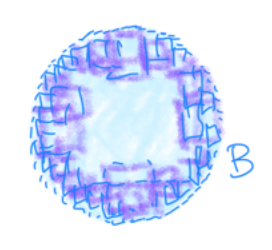
\includegraphics[scale=0.3]{images/base_rn} 
    \end{center}
    Pero también,
    \begin{center}
        
\includegraphics[scale=0.3]{images/bases_alternativas_rn} 
    \end{center}
    porque
    \[
    B\left( x, \varepsilon \right) = \bigcup_{i \in  I} cuadrados = \bigcup_{j \in J} rectangulos
    \]
\end{enumerate}
\end{ej}

\begin{pg}
    Como antes, a menudo basta considerar los abiertos de $\mathcal{B}$ 
\end{pg}

\begin{il}
$A \subset X$ denso $\Leftrightarrow \forall B \in \mathcal{B}, B \cap A \neq \emptyset$.
\end{il}

\begin{prop}
``$\mathcal{B} \subset \mathcal{P} \left( X \right)$ es base de una topología (única) $\mathcal{T}$ en $X$'' es equivalente a: 
\begin{itemize}
    \item $X = \bigcup_{B \in \mathcal{B}} B$.
    \item $\forall x \in B_1 \cap B_2,\ \exists B^x \subset B_1 \cap B_2$.
\end{itemize}
%TODO: Fix imagen
\begin{center}
    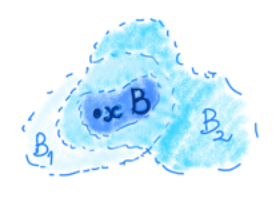
\includegraphics[scale=0.3]{images/base_unica} 
\end{center}
\end{prop}
%TODO: Mejorar
\begin{demo}
La implicación $\Rightarrow)$ se cumple por propiedades vistas.

En el otro sentido tenemos:
\begin{itemize}
    \item \underline{Unicidad}: $\mathcal{T} = \{\bigcup_{i \in  I} B_i: \{B_i\} \subset \mathcal{B}\}$.
    \item \underline{Existencia}: Esa $\mathcal{T}$ es efectivamente topología. 
        \begin{itemize}
            \item $\emptyset$ unión de vacío, $X = \bigcup_{i} U_i \Rightarrow \emptyset, X \in \mathcal{T}$.
            \item Uniones: $\bigcup_{j} \underbrace{\bigcup_{i} B_{ij}}_{\in \mathcal{T}} = \underbrace{\bigcup_{j} B_{ij}}_{\in \mathcal{T}}$. 
            \item Lo importante, intersecciones finitas: $B_1, B_2 \in \mathcal{B} \Rightarrow B_1 \cap B_2 = \bigcup_{x \in B_1 \cap B_2} B^x \in \mathcal{T}$.
            \begin{gather*}
                \forall x \in \left( \bigcup_{i} B_i \right) \cap \left( \bigcup_{k} B_k \right) \stackrel{?}{=} \bigcup_{\lambda} B_{\lambda}\\
                x \in B_{i_0} \cap B_{k_0} \Rightarrow \exists B^x \subset B_{i_0} \cap B_{k_0} \\
                \bigcup_{\lambda} B_{\lambda} = \bigcup_{x} B^x
            .\end{gather*}
        \end{itemize}
\end{itemize}
\end{demo}

\section{Topología relativa}%
\label{sec:topologia_relativa}
Sea $\left( X, \mathcal{T} \right)$ espacio topológico.
\begin{defi}
$Y \subset X: \mathcal{T}|_Y = \{U \cap Y: U \in \mathcal{T}\}$ es una topología en $Y$ (fácil), denominada \underline{relativa} ó \underline{restricción} a $Y$; también se dice que $\left( Y, \mathcal{T}|_Y \right)$ es un \underline{subespacio} de $\left( X, \mathcal{T} \right)$ y que $\left( X, \mathcal{T} \right)$ es el espacio \underline{ambiente}. 
\begin{center}
    %TODO: Fix imagen
    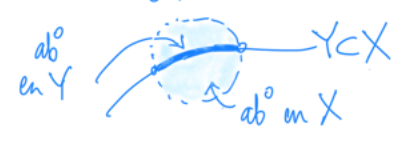
\includegraphics[scale=0.3]{images/def_subespacio_top} 
\end{center}
\end{defi}

\begin{obs}
\begin{enumerate}
    \item Los cerrados en $\mathcal{T}|_Y$ son $F\cap Y$ con $F$ cerrado en $\mathcal{T}$.
    \begin{demo}
    \[
    Y \setminus U \cap Y = Y \cap \left( X \setminus U \right) = Y\cap F
    \]
    \end{demo}
    \item 
    $\begin{cases}
        y \in Y \subset X\\
        \mathcal{V}^y \text{ base de entornos de } y \text{ en } \mathcal{T} 
    \end{cases}\Rightarrow \begin{cases}
        \mathcal{V}^y \cap Y = \{V^y \cap Y : V^y \in \mathcal{V}^y\} \\
        \text{base de entornos de } y \text{ en } \mathcal{T}|_Y 
    \end{cases}$

    \item $\mathcal{B}$ base de $\mathcal{T} \Rightarrow \mathcal{B} \cap Y = \{B \cap Y : B \in \mathcal{B}\}$ base de $\mathcal{T}|_Y$

    \item adh? int?
\end{enumerate}
\end{obs}

Esta idea es general: en un subespacio se hacen las construcciones intersecando.

\begin{ej}
\begin{enumerate}
    \item $y$ es un punto aislado de $Y \Leftrightarrow \{y\}$ abierto en $\mathcal{T}|_Y$.
    \begin{demo}
        $\exists U^y_{\text{ab.}}: \{y\} = U^y \cap Y$
    \end{demo}

    \item Todos los puntos de $Y$ son aislados $\Leftrightarrow \mathcal{T}|_Y = $ discreta.

    Se dice que $Y$ es un \underline{subespacio discreto}. 

    Por ejemplo, en $\mathbb{Z} \subset \mathbb{R}$:
    %TODO: Fix imagen
    \begin{center}
        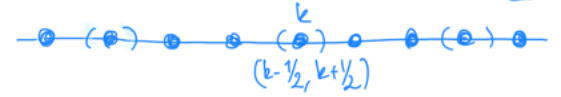
\includegraphics[scale=0.3]{images/def_subespacio_discreto} 
    \end{center}

    \item Sea $a \in X$ y $\mathcal{T}_a$. Entonces:

    La base mínima es $\mathcal{B} = \{\{a\} , \{a, x\}; x \in X\}$. Porque sea $B' \subset \mathcal{B}'$ (base), entonces como $\{a\} = \bigcup_{B'} B',\ \exists B' = \{a\}$ y, por otro lado, $\{a, x\} = \bigcup_{B'} B',\ \exists B': x, a \in B' \Rightarrow \{x, a\} = B'$ al ser $B'$ abierto. Con esto, los elementos de $\mathcal{B}$ están contenidos en todas las posibles bases.

    Por tanto, $a \in X, \mathcal{T}_a|_{X \setminus \{a\}} = $ discreta. Porque: $\mathcal{B} \cap Y = \{\{x\}: x \in X\setminus \{a\}\}$.

    \item Sea $W \subset Y \subset X$ con $W$ abierto/cerrado en $Y$ que es abierto/cerrado en $X \Rightarrow W$ es abierto/cerrado en $X$.

    \item Si $Y \subset X$ es abierto $\Rightarrow \mathcal{V}^a|_Y = \{V \cap Y : V \in \mathcal{V}^a\} $ es base entornos en $Y$ y en $X$.
    \begin{demo}
        Sea $(a \in ) W \stackrel{\text{ab.}}{\subset } X \Rightarrow a \in W \cap Y \stackrel{\text{ab.}}{\subset } Y \supset V \in \mathcal{V}^a|_Y$.

        Por otro lado, como $a \in V^a \Rightarrow \exists a \in U \subset V^a \subset Y$ abierto. Como $Y$ abierto $\Rightarrow U \subset X$ abierto $\Rightarrow V^a$ entorno de $X$.
    \end{demo}
\end{enumerate}
\end{ej}

\begin{obs}
\begin{enumerate}
    \item $Y \stackrel{\text{ab.}}{\subset} X: W \text{ abierto de } Y \Leftrightarrow W \text{ abierto de } X$ contenido en $Y$.
    \begin{demo}    
    \[
    W = U \cap Y^{\text{ab.}},\ U \stackrel{\text{ab.}}{\subset} X \Rightarrow W \stackrel{\text{ab.}}{\subset} X \text{ por intersección finita}
    \]
    \end{demo}
    \item $Y \stackrel{\text{cerr.}}{\subset} X: F \text{ cerrado de } Y \Leftrightarrow F \text{ cerrado de } X$ contenido en $Y$.
    \begin{demo}
    \[
    C = F \cap Y^{\text{cerr.}},\ F \stackrel{\text{cerr.}}{\subset} X \Rightarrow C \stackrel{\text{cerr.}}{\subset} X \text{ por intersección finita}
    \]
    \end{demo}
\end{enumerate}
\end{obs}
